\documentclass[a4paper]{article}

\usepackage[utf8]{inputenc}
\usepackage{erk}
\usepackage{times}
\usepackage{graphicx}
\usepackage[top=22.5mm, bottom=22.5mm, left=22.5mm, right=22.5mm]{geometry}

\usepackage[slovene,english]{babel}
\usepackage{hyperref}
\usepackage{url}

\let\oldfootnotesize\footnotesize
\renewcommand*{\footnotesize}{\oldfootnotesize\scriptsize}

\begin{document}
\title{Navodila in osnutek prispevka za končno poročilo pri predmetu Računalniška grafika}

\author{Blaž Rogelj 63150247$^{1}$, Luka Kadunc 63150136$^{2}$} % use ^1, ^2 for author(s) from different institutions

\affiliation{	$^{1}$Univerza v Ljubljani, Fakulteta za računalništvo in informatiko \\ 
				$^{2}$Univerza v Ljubljani, Fakulteta za računalništvo in informatiko }

\email{E-pošta: ciril.bohak@fri.uni-lj.si}

\maketitle

\selectlanguage{slovene}

\begin{abstract}{Abstract}
Naredila sva prvo/tretje osebno strelsko igrico. V igri se premikaš in uničuješ premikajoče se tarče. 
Igro lahko dokončaš tako, da pobiješ vse tarče ali pa porabiš vso strelivo.
V pomoč se v mapi nahaja paket z strelivom, ki ga je potrebno uničiti, da napolnimo svoje zaloge.
Igro sva naredila s pomočjo knjižnice BABYLON.

\end{abstract}

% -- Zgolj navodila - to v končni verziji dokumenta odstranite.
\section*{Navodila}
Ta dokument naj vam služi kot osnova za pisanje poročila o seminarju pri predmetu. Končno poročilo ne sme vsebovati več kot 4 strani besedila (skupaj s slikami lahko več), ne sme pa biti krajše od dveh strani vključno s slikami. Slike vključite v dokument kot kaže primer s sliko \ref{fig:slika} in se nanje tudi sklicujte. Prav tako v besedilu predstavite vsebino slik.

\begin{figure}[!htb]
    \begin{center}
        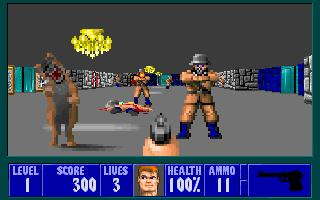
\includegraphics[width=\columnwidth]{wolfenstein.jpg}
        \caption{Kratek opis slike.} \label{fig:slika}
    \end{center}
\end{figure}

Pri pisanju poročila vključujte tudi reference na vire s katerimi ste si pomagali pri izdelavi seminarja. To so lahko pisni viri v obliki knjig \cite{Foley1994}, člankov \cite{Meng2015} ali drugih virov, ki jih dodajte med reference, spletne vire pa navajajte v nogi\footnote{\url{https://en.wikipedia.org/wiki/Computer_graphics}}.

Pri izdelavi igre se omejite na izdelavo enega samega nivoja igre, ki pa ga dodelajte in izpilite kolikor vam do\-pu\-šča predviden čas.

% do sem gre ven



\section{Pregled igre}
Igra je bila sprva mišljena kot tretje osebna, vendar sva se zaradi problemov pri uvozu karakterjev, ki nosijo orožje odločila, da bova naredila prvo osebno.
Sprva nama je uspelo uvoziti karakter, ki je bil brez orožja. Uspelo nama ga je animirati in narediti njegovo premikanje.
Težava je bila v tem, da naš karakter ni imel orožja, zato sva se odločila uvoziti nov model z orožjem. 
Pretvorba ob mnogih poizkusih z drugimi tipi in modeli (ki so vsebovali animacijo premikanja) v .babylon format žal ni bila uspešna.
Ker pa nisva želela zavreči tega kar sva do sedaj naredila lahko igro igramo v dveh načinih. Prvo osebnem in tretje osebnem.
Igra ni zahtevna izgubiš jo lahko le, če namerno trošiš strelivo. Težavnost igranja, bi se dalo preprosto zvečati, če bi povečali hitrost tarč, ki se premikajo v okolju.
Pri streljanju moramo meriti malo pred tarčo, če jo želimo zadeti. Naboji niso neskončno hitri in potrebujejo nek čas, da priletijo do tarče.
Igra je namenjena vsem ljudem, ki jih zanimajo strelske igrice.


\subsection{Opis sveta}
Naš svet je 2D ravnina, po katerem se premikamo le v 2D. Nad ravnino lebdijo sfere. Sfere predstavljajo sovražnike, ki jih moramo uničiti.
Ko zadenemo našo tarčo ta izgine kot tudi naboj, ki jo zadene. Če zgrešimo naš naboj odleti v neskončnost in nato izgine.

\subsubsection{Pregled}
Naš svet je omejen s štirimi stranicami, ki preprečujejo padec ven. Po svetu kroži več sfer. Njihovo število je odvisno od težavnosti, kot tudi
število nabojev. V mapi nas vedno pričaka natanko en paket z dodatnim strelivom. Ko zadanemo sfero, bo ta izginila.

\subsubsection{Ozadje}
Za ozadje sva postavila sliko mesta z temnejšo grafiko, da se bolje zlije z vzdušjem igre. Slike so vpete na 6 stranic velikega kvadra, ki objema cel naš svet.

\subsubsection{Ključne lokacije}
Lokacija, ki je pomembna za uporabnika je polje kamor se zgenerira naš paket streliva. Ko ga uporabnik pobere ta izgine in se ob tem predvaja tudi zvok. 
Generiranje sfer se dogaja v svetu na naključnih lokacijah. Vsaka sfera lebdi po neki svoji začrtani krožnici. 
Radij kroga po katerem krožijo je enako velik za vse sfere.

\subsubsection{Velikost}
Velikost sveta v katerem se nahaja naš uporabnik, je statična in se z igranjem ne spreminja. Na robu stranice nas iz vseh štirih strani omejuje zid, ki preprečuje padec iz mape.

\subsubsection{Objekti}
Glavni objekti v igri so:
-naše orožje
-sfere ki predstavljajo tarče
-naboji ki odletijo, ko sprožimo akcijo streljaj
-zaboj z dodatnimi naboji

\subsubsection{Čas}
Z časom se v naši igri spreminja le pozicija tarč.

\subsection{Igralni pogon in uporabljene tehnologije}
Igra je napisana v javascriptu s pomočjo knjižnice BABYLON. Poleg tega sva uporabila tudi Blender za pretvorbo različnih 3D modelov v .babylon format. 
Pred blenderjem sva uporabila še Autodesk, vendar se ni obnesel najbolje.

\subsection{Pogled}
Naša kamera je ArcRotateCamera. Pogled na igro je lahko prvo oseben ali tretje oseben z pritiskom na tipko V


\section{Osebek}
Naš osebek je nek karakter, ki nosi pištolo. Premikamo ga lahko naprej ali nazaj z tipkama W in S. Z miško ga lahko obračamo, vendar moramo pred tem z miško pritisniti, da karakter postane aktiven.
Osebkove akcije
-streljaj ob levem kliku miške
-ob pritisku na R napolni orožje
-ob pritiski na V spremeni pogled


\section{Uporabniški vmesnik}
Na začetku igre se nam pojavi glavno okno za pričetek igre. Tam moramo obvezno izbrati težavnost in pritisniti Save gumb, če tega ne storimo ne dobimo nabojev ob pričetku igre.
Ko se igra prične moramo pritisniti z miško, da canvas postane odziven. Da dobimo nadzor nad miško nazaj moramo pritisniti tipko escape. 
Ob igranju nam v zgornjem levem kotu prikazuje koliko nabojev imamo v magazinu in koliko metkov imamo na sploh. Na zgornjem desnem kotu pa imamo gumb za izhod, če želimo končati igro.
Če ga želimo pritisniti moramo najprej klikniti escape.


\section{Glasba in zvok}
V naši igri je implementiran zvok, ki se predvaja ob strelu in zvok, ki se predvaja ob polnjenju nabojev. Pridobila sva ga iz KADUNC DOPOLNI. 

\section{Gameplay}
Z tipkama W in S se lahko premikamo naprej in nazaj. Ob levem kliku miške streljamo. Ko nam zmanjka streliva, ga napolnimo z črko R.
Če nam streliva začne primanjkovati lahko uničimo paket, da ga pridobimo nazaj. Da tarčo zadenemo, moramo meriti malo pred njo, ker naboji potrebujejo nek čas,
da priletijo tja. Igro zmagamo tako, da pobijemo vse tarče, ki lebdijo. Če nam tega ne uspe igro žal izgubimo.
Za spremembo načina igranja pritisnemo črko V. Na črko L je še implementirana skrita akcija.



\section{Zaključki in možne nadgradnje}
Naučila sva se osnove računalniške grafike in delo z knjižnico Babylon. Da bi igro napisala, kot je bil njen predviden scenarij sva tekom semestra pridobila dovolj znanja.
Razlog, da igre nisva napisala po predvidenem scenariju je bil pomanjkanje časa.
Razlike ki so nastale:
-nisva naredila življenja našega karakterja in medicinskih paketkov
-manjka mu še pobijanje z drugimi tipi orožja
-nisva naredila seštevanja točk, ki nam lahko prinesejo različne nadgradnje
-tarče te ne morejo poškodovati



\small
\bibliographystyle{plain}
\bibliography{references}

\end{document}
